\chapter{Some physics}\label{ch:physics}



When I was an undergrad, I majored in both math and physics. Through my math
major I learned some useful things about how mathematical structures work on a
fundamental level. However I think my math major was detrimental to my
understanding of physics philosophy. In math, you start with some rules or {\it
axioms}, and {\it formally derive} everything from that using logic only. 
These derivations are organized as proofs. I found it pretty satisfying to 
come to the end of a proof, because I felt like I had some airtight, undeniable 
knowledge about something. 

Physics is not really the same, in that physicists will often 
use facts that cannot be derived in that way. These facts come from
observing the world, which is usually accomplished via experiments.
For instance, the laws that govern electrodynamics, {\it Maxwell's equations},
are known through observation. More sophisticated theories from which one
can ``derive" Maxwell's equations {\it were tailored in part to achieve that
end}. If you think about it this makes sense: If you already know that Maxwell's
equations are true, then if you want to make a more sophisticated theory, you
better at least recover Maxwell's equations. 
Comparison of our ideas with experiment is viewed as the ultimate check.

Let me introduce some terminology. By {\it model}, I will mean roughly ``the
ideas we have about how the world works." A model is just a way of thinking
about reality. There is nothing that forbids two models from describing the same
reality\footnote{Provided that the models don't contradict each other in some
way.}. Models have observations at their foundation, and they are extended using
logic and sometimes assumptions. Sometimes these extensions will tell you
something quantitative about a natural phenomenon that you are not currently
observing or a phenomenon that has not yet been observed: this is a {\it
prediction}. If a prediction agrees with experiment, it lends credence to our
model, and by extension to our assumptions, if we made any.
In my view, {\it models are not any more real than that}. 
They are a faithful description of reality exactly to the extent that they 
agree with observations and yield correct experimental results.

That may make you feel uncomfortable or feel ambiguous, but I find it
empowering. First of all at least in physics, accepted models yield extremely
precise precisions that turn out to be accurate. Secondly, it gives physicists
some leeway when developing and understanding their models. We are free
to use assumptions that will make our calculations easier, and we are free to
think about reality however we like, {\it as long as we ultimately obtain quantitative
results that agree with experiment, and as long as our models are free of
contradictions}.

In the following, I am going to introduce some basic ideas in physics that I
think are necessary to have some understanding of lattice field theory.
Some of these ideas about reality may seem
counterintuitive, uncomfortable, or bizarre. Nevertheless, these ideas, these
ways of thinking about things, seem to be correct, again because they eventually
produce highly precise quantitative predictions that are vindicated in
experiment time and time again. 


\section{Units and dimensional analysis}


Measurements have units, and therefore units are of fundamental importance when 
interpreting things in physics. They are so important, that I like to set them off 
with square brackets []. For instance all distances can be measured in [mi] (miles), 
all times in [h] (hours), all weights in [lb] (pounds), and so on. 
Besides connecting numbers to the natural world, units are an opportunity to
check for errors. Once you have settled on a {\it unit system}, which I will
discuss more in \secref{sec:units}, two guidelines you can use are
\begin{enumerate}
  \item A physical quantity cannot change its units over the course of a
        calculation. For instance, how far away we are from the sun must always
        have units of distance.
  \item You can only add and subtract physical quantities with matching units.
        For instance, it makes no sense to add an [h] to a [lb].
\end{enumerate}
If you find you have done one of these things at some point during a
calculation, you have made a mistake.

You can, however, always multiply and divide units. A common example is the 
following: If you are driving and manage to travel 20 [mi] in 1 [h], then your speed is
\begin{equation}
\text{speed}=\frac{20\units{mi}}{1\units{h}}=20\units{mi/h}.
\end{equation}
In this example, we see that we can build new physical quantities\footnote{We
also sometimes call quantities that can be measured {\it measurable quantities} 
and {\it observables}.}, in this case the speed, out of other physical quantities; 
correspondingly we can build new units out of old ones. 

I picked the units [mi] and [h] to create the speed because this is what we Americans 
are used to. However in the scientific community, we tend to measure distance in 
meters [m] and seconds [s]. This brings us to another important skill: We need to be 
able to convert between different units when measuring the same observable.
This conversion is called {\it dimensional analysis}\index{dimensional analysis}.

To do that, we need to answer two questions: How many [m] are in a [mi]? How many [s] 
are in an [h]? It’s usually not worth memorizing such things\footnote{You can
sometimes gain physical intuition by memorizing such conversions.}.
If I do a quick Google search, I find
\begin{equation}
1\units{mi}=1609\units{m}~~~~\text{and}~~~~1\units{h}=3600\units{s}.
\end{equation}
To do the conversion, we will now multiply a chain of unit ratios, each ratio containing 
units for the same kind of observable, such that the numerator of one ratio cancels 
the denominator of the following one. So for example with speed, that will look like
\begin{equation}
\frac{20\units{mi}}{1\units{h}}
\frac{1609\units{m}}{1\units{mi}}
\frac{1\units{h}}{3600\units{s}}
\approx8.9\units{m/s}.
\end{equation}

\subsection{Mass vs. weight}
Apropos the imperial units/metric units rivalry, you may have noticed that the US reports 
weights in [lbs], while others report it in [kg]. However, this difference in units is not 
exactly the same as with distance or time; actually [kg] is a measurement of mass 
and [lbs] is a measurement of weight. A weight is a type of force; generally speaking 
forces are things that push or pull. Weight in particular refers to the force of 
gravity that you feel on the earth. Its magnitude $w$ is given by
\begin{equation}\label{eq:weightMass}
w=mg,
\end{equation}
where $m$ is the mass and $g$ is the acceleration due to gravity, which is
\begin{equation}
g=9.8\units{m/s$^2$}
\end{equation}
Since the units of mass are [kg], the units of weight must therefore be
\begin{equation}
[w]=\frac{\units{kg}\units{m}}{\units{s$^2$}}\equiv\units{N},
\end{equation}
where the RHS gives the familiar Newton, our typical unit of force.

Technically speaking forces and masses are not the same kinds of physical quantities.
Still, \equatref{eq:weightMass} shows us that even though they are not the same 
kind of physical quantity, they are not really different either; i.e. {\it they are the 
same up to a constant}\footnote{In actuality, $g$ is not a constant. In fact, it
depends on the earth’s mass and how far away you are from the earth’s center. We
are treating it as a constant because the difference in $g$ between, say, the
first floor and top floor of the Empire State Building is so small that you can
ignore it for most calculations. In introductory physics classes, they usually
take great care to distinguish between mass and weight. This is because your
mass is completely independent of your distance from your distance to the
earth’s center. As another example, $g$ on the moon’s surface is much smaller than
$g$ on the Earth’s surface, because the Earth is much more massive than the moon.
A consequence of this is that astronauts on the moon are much lighter than on
the Earth, i.e. they have a smaller weight.}, in this case, $g$. 
This effective equality between weight and mass is utilized when 
Europeans report weights in [kg].


\section{Energy}\index{energy}
Imagine any physical object at all; it does not matter what it is. 
Energy is our attempt to quantify either
\begin{enumerate}
    \item That object doing something, like moving around, deforming, breaking, 
          getting hotter, making noise, and so on; or
    \item The potential for that object to do one of the above things.
\end{enumerate}
The second of the above is usually called {\it potential
energy}\index{energy!potential}. To get some intuition for potential energy, 
imagine holding a ball. What will happen if you let go of it? The fact that the 
ball will fall when you let go demonstrates that it has some potential energy, 
in this case gravitational potential energy.

A mnemonic way to think about energy is that it can flow into and out of things. 
For instance, let’s imagine we’re at the gym, and we want to pick up a dumbbell.
The dumbbell’s not moving, it’s not hot, it isn’t making any noise, it’s on the
ground--we think of this dumbbell as having no energy. If the dumbbell were above the
ground, it would have some potential energy. Therefore if you want to raise the
dumbbell, you have to add some energy to the dumbbell 
system\footnote{One of the trickiest parts of problem solving is isolating in
your mind the only things that are relevant to that problem. In physics, we call
that collection of things we want to think about a {\it system}\index{system}. 
Usually there is more
than one correct way to solve a problem; correspondingly there may be more than
one correct way to think about things, i.e. more than one useful system to
imagine. I can’t think of a well defined way to pick systems. It is something
you just have to get the hang of. We are constantly finding new ways to think
about things, so don’t stress out too much about finding the perfect way to
imagine things. You only have to find a way of imagining things that’s good
enough to solve the problem at hand.}, and if you like, you can think about energy 
flowing out of you and into the dumbbell as you raise it.

Let’s try to be quantitative about this process: How much energy will it take to
raise a 10 [kg] dumbbell by half a meter? Well, the more massive it is, the
more energy it should take. Also the stronger gravity is, the more energy it should
take. Finally the higher you need to lift it, the more energy it should take. A
formula that captures all of this, and what you've likely already
learned\footnote{I'm belaboring these basic ideas a little because I want you to
see an example of the kind of reasoning you might do to discover such a formula
in the first place.}, is 
\begin{equation}\label{eq:gravpot}
E=mgh,
\end{equation}
where $E$ is the energy and $h$ is how high you lifted it off the ground.
Therefore lifting the dumbbell takes
\begin{equation}
10\units{kg}\times9.8\units{m/s$^2$}\times0.5\units{m}=49\units{kg~m/s$^2$}\equiv49\units{J},
\end{equation}
where we have introduced the Joule, the familiar unit of energy.

To finish this section, we report a relationship between energies and certain
kinds of forces. Roughly, a {\it conservative force}\index{force!conservative} 
is a force that conserves mechanical energy, i.e. it does not lose energy to heat or
vibration\footnote{This is an informal definition. A better definition is that
a force is conservative if the work it does is path-independent. But to
understand that definition I would have to introduce line integrals, which I
wanted to avoid.}, when you move in a line along the force field. 
For such forces there exists a well defined potential energy
$U$ which is related to the force by
\begin{equation}
F=-\dv{U}{r},
\end{equation}
where $r$ is the distance along the force field you moved. Consider the above
example of gravity near the earth's surface. Here the force field is
perpendicular to the floor, and the height $h$ off the floor is the distance you
move parallel to the force field. Using the expression for gravitational
potential energy \eqref{eq:gravpot}, we find for the gravitational force
\begin{equation}
F=-\dv{(mgh)}{h}=-mg,
\end{equation}
i.e. gravity points down with a magnitude $mg$, as you already knew.

\section{Aspects of electrodynamics}\label{sec:EM}

Electricity and magnetism are ubiquitous in modern life. Indeed, I am right now sitting 
in an airport glowing with screens and lights, typing notes on a laptop. Busy
people are communicating long distance with their cell phones, their
conversations punctuated by loudspeakers delivering flight information.

The basic principles of electromagnetic (EM) phenomena are straightforward.
Some particles carry an {\it electric charge}\index{charge!electric}, which can
be positive or negative. The most familiar is the electron, whose charge is
defined to be -1. When two particles have the same charge, they repel, and when
they have opposite charges, they attract. We conclude that charged particles
exert some kind of force on each other. Moreover the force is weaker the farther
away you are. These ideas are summarized in {\it Coulomb's law}\index{Coulomb's
law},
\begin{equation}\label{eq:coulombForce}
\vec{F}=\frac{q_1 q_2\hat{r}}{4\pi\epsilon_0 r^2},
\end{equation}
which gives the force between two particles of charges $q_1$ and $q_2$,
separated by a distance $r$. The $\hat{r}$ tells us that the force points along
the line connecting the two particles. $\epsilon_0$ is a constant called the {\it
vacuum permittivity}\index{vacuum permittivity}. We imagine the cause of this
force to be an {\it electric field} $\vec{E}$. For instance if we imagine a
system with only the source charge $q_1$, its electric field is
\begin{equation}
\vec{E}=\frac{q_1\hat{r}}{4\pi\epsilon_0r}.
\end{equation}
Viewed in this way, \equatref{eq:coulombForce} is the force a test charge $q_2$
would feel if placed at a position $r$ in the field generated by $q_1$.

The Coulomb force turns out to be a conservative force. From the logic of the
last section, its corresponding potential energy is
\begin{equation}
U=\frac{q_1 q_2}{4\pi\epsilon_0 r}.
\end{equation}
The analogue to the potential energy for the electric field is the so-called
{\it electric potential},
\begin{equation}
V=\frac{q_1 }{4\pi\epsilon_0 r},
\end{equation}
whose unit is the {\it volt}\footnote{This is not a very helpful definition of a
volt. To give a better definition, however, is 
a bit of a digression. I just want to give you a conceptual introduction to
this quantity so that it makes some sense to relate it to energy.} (V).
The amount of energy it takes to push an electron through one volt defines
another unit, the {\it electron-volt}\index{electron-volt} [eV].

The electron-volt is extremely useful as a unit of energy in the context of 
particle physics experiments. One of the most common ways to learn something about 
particles is to collide them with each other. This requires accelerating a
particle, which is typically done by placing it in an electric field.
In this experimental environment, back when the commonly accelerated particle was an
electron, it was likely natural to think of the imparted energy in
terms of [eV]. It seems to have stuck as a convention since those times.

Finally I mention that electricity and magnetism are actually both
manifestations of the same phenomenon, which is sort of suggested already by the
name ``electromagnetism". In particular, it turns out that magnetic fields are
caused by moving charges. For instance two unshielded, current-carrying wires
parallel to each other will attract or repel each other depending on the
direction of that current.

\section{Aspects of special relativity}\label{sec:SR}\index{relativity!special}

Everything I discussed up to now, you may have already seen, and probably none
of it is surprising. This will be the first section where I introduce some 
ideas that more likely to be uncomfortable. 

The core idea of {\it special relativity} is that the speed of light $c$ is completely independent 
of everything\footnote{More precisely, the statement is that ``the speed of light in a 
vacuum is the same in all inertial reference frames". You don't have to know exactly 
what this means. I am just putting this here so you know I haven’t given you the full 
story. To give you the full story is a bit too much of a technical digression for the 
purpose of these notes.}. 
It doesn’t matter where in the universe you are, it doesn’t matter what is 
nearby, it doesn’t matter what the temperature is. In all of these cases, the speed of light 
is the same. One can show that a consequence of this fact\footnote{You have to
assume {\it causality}\index{causality}, which means that if event $A$ {\it
causes} event $B$, it must occur {\it before} event $B$ in all reference
frames.} is that $c$ is the largest possible speed.
It turns out that light travels in little packets called {\it photons}.

An immediate consequence of this is a relationship between distance and time. In particular 
if a photon travels for a time $t$, it will always traverse a distance
\begin{equation}
d=ct.
\end{equation}
Revisiting our logic about weight and mass, this tells us distance and time are not 
really different\footnote{In fact, the logic is even stronger for the
distance/time equivalence, since the speed of light in a vacuum really is a
constant, unlike g in the example of weight and mass.}. This is especially
useful for astronomical distances: You have probably heard of the lightyear [ly],
which is the distance a photon travels in a year [y].

To get a handle on how far a [ly] is, we need to know $c$, which is
\begin{equation}
c\approx3\times10^8\units{m/s}.
\end{equation}
Then, using the dimensional analysis we learned before, we find
\begin{equation}
1\units{ly}
\approx3\times10^8\frac{\units{m}}{\units{s}}\times1\units{y}
\times\frac{3.154 \times 10^{7}\units{s}}{1\units{y}}
=9.462 \times 10^{15}\units{m},
\end{equation}
which is about ten-thousand-million-million [m]. Besides the sun, the nearest
star to us is Proxima Centauri, which is about 4 [ly] away.

This time-distance equivalence is even more profound than that. Think about
where you are sitting right now. You can imagine in your mind a coordinate
system in three dimensions, whose origin is located on the chair you're sitting
on. You can move with respect to that origin, either forward-backward
($\hat{x}_1$-direction), left-right ($\hat{x}_2$-direction), or up-down 
($\hat{x}_3$-direction); this is what it means to exist in three dimensions.
The time-distance equivalence allows us to define a fourth dimension,
the $\hat{x}_4$-direction, where\footnote{Usually this coordinate is labelled as
$x_0$. In LFT we call this coordinate $x_4$.} $x_4\equiv ct$. Note that this has units of
distance, so it makes sense to put them all in the same set of axes. Now think about
your chair again, which was the origin of our 3-$d$ system, and define this very
moment right now to be $x_4=0$. This defines an origin for our 4-$d$ system,
which we call {\it space-time}. If you don't move in the 
$\hat{x}_1$-, $\hat{x}_2$-, or $\hat{x}_3$-directions, i.e. if you sit still,
you are moving in the $\hat{x}_4$-direction, and in that way trace out a curve
in space-time called a {\it world-line}.

So when we think about reality from now on, its domain will be
$\R^4$, which is defined by \equatref{eq:spacetimeSet}.
In physics parlance, any function that depends on your location in space and
time is called a\index{field} {\it field}\footnote{In math parlance, 
``field" has another meaning.}. For example, everywhere in the universe, at
every time, there is a temperature. This defines a {\it temperature field},
\begin{equation}
T:\R^4\to\R.
\end{equation}
Since the codomain of $T$ is $\R$, it is a {\it scalar field}\footnote{If you
take an advanced course in relativity, or when you take quantum field theory in
grad school, you will learn a slightly more specialized definition of ``scalar".
We won't discuss that definition. Still I wanted to leave this footnote so I
wouldn't feel guilty about lying to you.}.

I would like to introduce one more equivalence to you, the energy-mass
equivalence. This is summarized by what is perhaps the most well known equation
in all popular culture,
\begin{equation}\label{eq:emc2}
E=mc^2,
\end{equation}
where again $E$ is energy and $m$ is an object's mass.
This is also a consequence of relativity. Again returning to our weight/mass or
distance/time logic, it follows that energy and mass are not really different.
Earlier we said that energy means an object is doing something, or it has the
potential to do something. Einstein showed us that, in addition,
\begin{enumerate}
\setcounter{enumi}{2}
\item anything with mass, even if it’s just sitting there, also has energy.
\end{enumerate}
In other words, it would cost some energy to generate two apples out of the
void. This is called the apples’ {\it rest mass energy}\index{energy!rest mass}.

There are some even more interesting consequences of special relativity, which I
hope you look forward to in your modern physics class, or which I encourage you
to look into on your own. For the purpose of these notes, I think I have covered
enough to get some basic intuition for LFT.


\begin{figure}
  \centering
  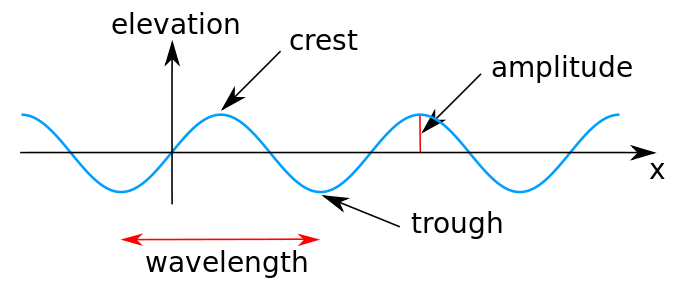
\includegraphics[width=\linewidth]{figs/wave.png}\\
  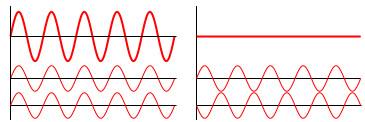
\includegraphics[width=\linewidth]{figs/interference.png}
  \caption{{\it Top}: A simple wave. Local maxima are referred to as {\it
crests}\index{crest} while local minima are {\it troughs}\index{trough}. The
distance between crests is the {\it wavelength}\index{wavelength}. The crest
height is the {\it amplitude}\index{amplitude}. Image taken from
Wikipedia~\cite{wiki:wave}.
{\it Bottom}: Constructive (left) and destructive (right) interference. 
The top wave is created by adding together the bottom two. For example let us
say that the amplitude of the bottom waves is 1 in some units. In the
constructive case, two crests appear at the same point, and so the crest of the
resultant wave will be $1+1=2$. In the destructive case, a crest and trough
appear at the same point and cancel. Image taken from
Wikipedia~\cite{wiki:interfere}.
}
  \label{fig:wave}
\end{figure}

\section{Aspects of quantum physics}\label{sec:QM}

One of the first physical phenomena to reveal to us the extraordinary nature of
short-distance physics was light. Light had been studied for centuries, with
important advances in its understanding coming from the likes of Euclid, Alhazen,
Young, Newton, and Huygens. Through Young and Huygens, light was understood to 
be a {\it wave}\index{wave}, which we will think of in these notes as some function on
space-time that is periodic in space or time or both. A sketch of a simple wave,
along with some related vocabulary is shown in \figref{fig:wave} (top).

Waves represent some kind of departure from an equilibrium state; put another
way, a real wave of one variable with no change from equilibrium would be just 
a straight horizontal line. Departures from equilibrium cost energy, so
intuitively, you can imagine that the more wiggly a wave is, the more energy it
has. A more wiggly wave has a shorter wavelength, so we can intuitively expect
an inverse correlation between the energy of a wave and its wavelength.
When two waves are superimposed on each other, they {\it
interfere}\index{interference}. If the waves mostly work together, they interfere {\it
constructively}, whereas if they mostly cancel each other out, they interfere
{\it destructively}. Examples of totally constructive and totally destructive
interference of a simple way if shown in \figref{fig:wave} (bottom).

To learn that light is a wave, Young performed a {\it double-slit
experiment}\index{double-slit experiment}. The idea is that one shines light
through two small slits in a wall, which then strikes some screen behind the
wall. If light were not a wave, one would expect to see two lit spots on the
screen, directly behind the slits. Instead, what Young found was an interference
pattern like shown in \figref{fig:twoSlit} (top). This {\it interference
pattern}\index{interference!pattern} if light is a wave. A rough explanation of
how that works is depicted in \figref{fig:twoSlit} (bottom).

\begin{figure}
  \centering
  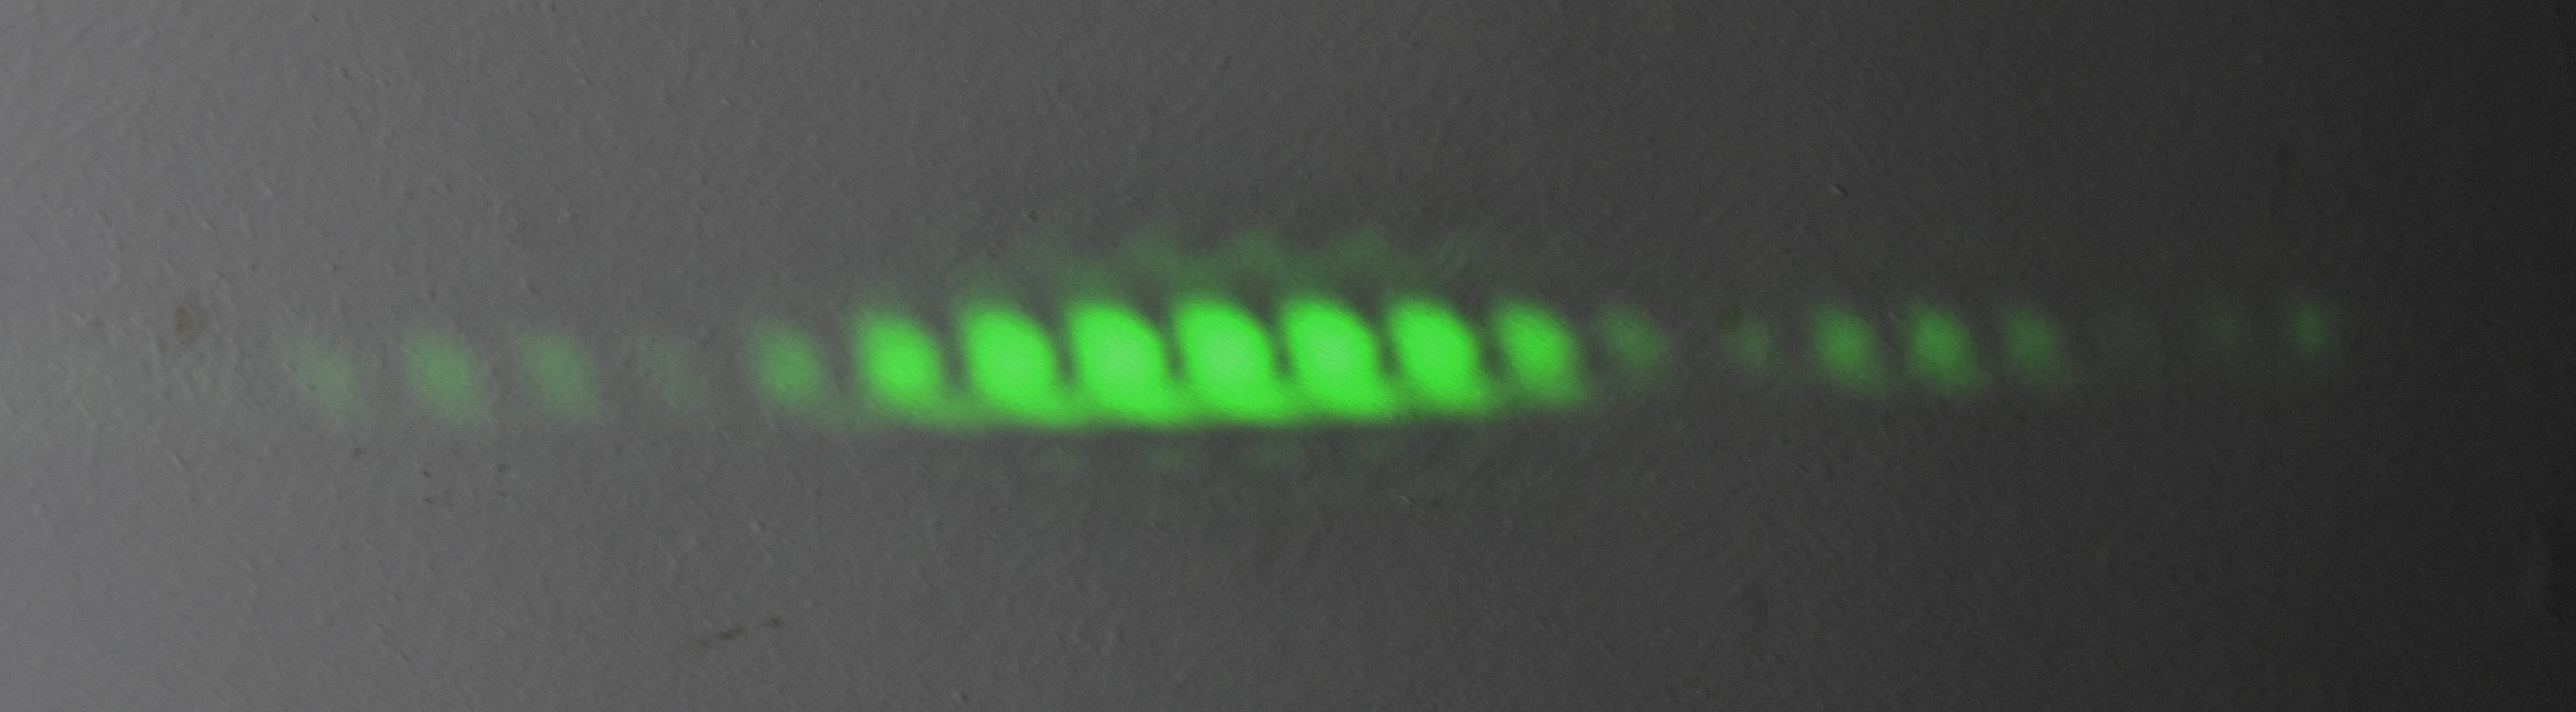
\includegraphics[width=\linewidth]{figs/Youngs_slits.jpg}\\
  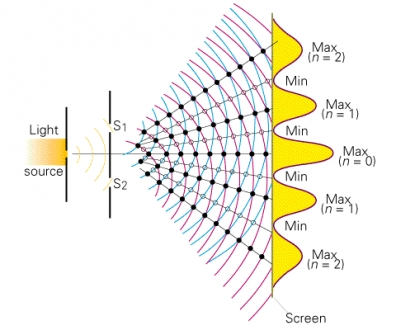
\includegraphics[width=\linewidth]{figs/twoSlitMechanism.jpg}
  \caption{{\it Top}: An example interference pattern one sees when shining green light
through two nearby slits. Image taken from Wikipedia~\cite{wiki:slit}.
{\it Bottom}: Diagram showing the mechanism behind interference patterns. S$_1$
and S$_2$ indicate the slits. The blue and red circle segments indicate maxima
of the waves coming from S$_1$ and S$_2$, respectively. Places where the circle
segments intersect yield complete constructive interference; when these segments are
instead evenly separated, a crest coincides with a trough, giving
complete destructive interference. Image taken from Ref~\cite{deutsch:slit}.}
  \label{fig:twoSlit}
\end{figure}

In the early 1900s, physicists were beginning to see the particle nature of
light. In particular, Planck proposed~\cite{Planck:1901tja}
that light may deliver {\it discrete packets} of
energy, rather than delivering a continuous spectrum of energy\footnote{He was
inspired to propose this because it avoided the\index{ultraviolet catastrophe}
{\it ultraviolet catastrophe}, which is the fact that light with a continuous
energy spectrum and arbitrarily
small wavelength has arbitrarily high intensity, i.e. its intensity diverges.}.
Under Planck's suggestion, light should only be able to have integer multiples
of some set amount of energy, with no other energies possible. Another way we
physicists say this is that the energy must be {\it quantized}. Planck wasn't
sure how this quantization occurred, suggesting for example that perhaps the
walls of a material absorbing light can only absorb quantized energy packets,
for some reason.

Einstein took Planck's idea seriously~\cite{Einstein:1905cc}
and used it to explain the {\it photoelectric
effect}\footnote{This is actually what won Einstein the Nobel, not special or
general relativity. Also in 1905 he published his first
papers on special relativity, as well as a paper on Brownian motion.},
which is the observation that shining light on a material frees electrons. 
In fact, Einstein proposed that this quantization was due to light itself, 
suggesting that light comes
in discrete energy packets. These are the {\it photons}\index{photon}.
A careful study~\cite{millikan_direct_1916} of the photoelectric effect by
Millikan showed that
Einstein's interpretation explained the photoelectric effect well. Finally
Compton showed that light scattered from a particle shifts by the Compton
wavelength\index{wavelength!Compton}
\begin{equation}\label{eq:compton}
  \lambda_c=\frac{\hbar}{2mc},
\end{equation}
where $m$ is the target particle's mass, and $\hbar$ is a constant called
{\it the reduced Planck constant}\index{Planck constant}, 
which one can derive by assuming light
is made of particles with zero rest mass~\cite{Compton:1923zz}.
Altogether these discoveries convinced physicists light behaves as a particle
at short enough length scales. 

As hinted by \equatref{eq:compton}, something else interesting became apparent
around this time: Particles such as electrons also behave like waves. For
example one can carry out the double-slit experiment with electrons, which are
also seen to exhibit interference patterns. Equation~\eqref{eq:compton} assigns
a characteristic wavelength to every particle. Repeating once again the logic of
previous sections, that $\hbar$ and $c$ are constants of nature suggest that
wavelengths and inverse masses can be thought of as ``the same".
This observation that light and matter particles such as electrons can behave as
particles or waves depending on the energy led us to believe that all particles
behave also as wave, a concept called {\it wave-particle
duality}\index{wave-particle duality}. This duality, along with the existence of
discrete energy levels, are two properties of quantum mechanics.


\begin{figure}
  \centering
  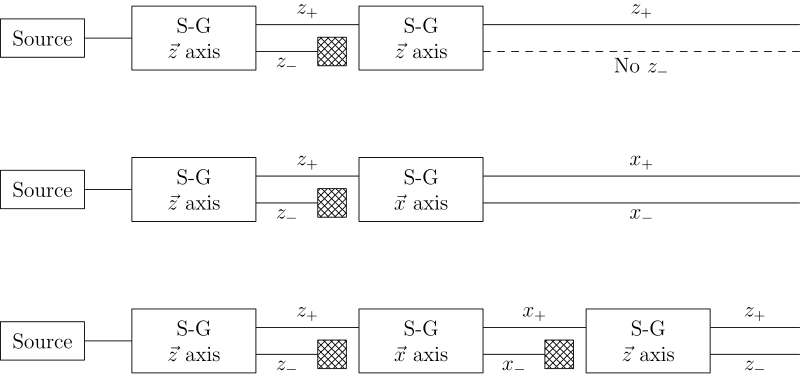
\includegraphics[width=\linewidth]{figs/stern-gerlach.png}
  \caption{Schematic representation of the Stern-Gerlach experiment.
           {\it Top}: A particle has its spin measured along the $\hat{z}$-axis,
which is found to be $+1$. Subsequent measurements along the $\hat{z}$-axis 
will always find +1. {\it Middle}: A particle has its spin measured along the
$\hat{z}$-axis, followed by the $\hat{x}$ axis. The $\hat{x}$-axis spin is
either +1 or -1 with probability 0.5 in each case. {\it Bottom}: A particle has
its $\hat{z}$-axis spin measured, which is found to be +1. A measurement along
the $\hat{x}$-axis destroys our knowledge of its spin, and the following
measurement along the $\hat{z}$-axis is again either +1 or -1 with probability
0.5 in each case. Image taken from Wikipedia~\cite{wiki:SG}. }
  \label{fig:sternGerlach}
\end{figure}

One of the earliest, most important experiments for quantum systems 
was the celebrated Stern-Gerlach
experiment~\cite{gerlach_experimentelle_1922a,gerlach_magnetische_1922b,gerlach_experimentelle_1922c}.
In this experiment, silver atoms were deflected by a magnetic field, which was
used to measure the {\it spin}\index{spin} of the atoms. In general, a
particle's spin is somewhat like its angular momentum\footnote{This statement
comes from the fact that the mathematics for angular momentum and spin are the
same in quantum physics. Physically we understand magnets as follows: Their
magnetic fields are due to the contributions of the spins of all the particles
in the magnet.}, hence the name. A particle's spin influences how it 
interacts with electromagnetic fields. A rough schematic of the Stern-Gerlach
experiment is given in \figref{fig:sternGerlach}.

As suggested in the caption of \figref{fig:sternGerlach}. The Stern-Gerlach
experiment suggests a fundamental randomness to particles. In paricular if you
have a particle, you can't generally predict\footnote{You may wonder if this
randomness is a ``true" randomness, or whether it stands in for some missing
information. For instance if you toss a coin, if you know the exact shape of the
coin, its weight, air resistance, the exact starting position of your hand,
the exact power and path of your throw, and so on, then in principle you can predict how 
the coin will land. It is natural to guess that quantum physics is the same,
that there is some as-yet-underdiscovered hidden information that would allow us
to predict the outcome of a quantum experiment, if only we knew it. If you did
guess this, you'd be in good company, since this 
is what Einstein thought. This hidden information is usually called a {\it
hidden variable}\index{hidden variable} in this context. In the 1960s, Bell
argued on rather general grounds that quantum physics without a hidden variable
must satisfy a certain inequality, which we now call {\it Bell's
inequality}\index{Bell's inequality}~\cite{bell_einstein_1964}. 
Fascinatingly in the early 1980s, Aspect, Grangier, and Roger confirmed Bell's inequality
experimentally~\cite{aspect_experimental_1982}, which is why they got the 2022
Nobel prize. The most likely scenario
therefore appears to be that there is no hidden variable, which means that fundamental
reality is in this sense truly random. Indeed quantum systems are the only
truly random things we are aware of. Other things that appear random, such as
random number generators, are actually deterministic at their foundation.
For completeness, I would like to mention that there are technically ways around 
Bell's inequality. Some of these ways have already been experimentally ruled
out. One possibility that has not yet been ruled out, but which also appears to
not be nearly developed enough to provide experimental predictions, is {\it
superdeterminism}\index{superdeterminism}. A superderministic theory would
underlie quantum mechanics, and my understanding of superdeterminism is that all
experimental outcomes in all space-time should at least in principle be tracable
back to one single set of initial conditions.} 
its $\hat{z}$-component of spin,
unless it has been specially prepared\footnote{In the context of the
Stern-Gerlach experiment, ``specially prepared" means you just took a
measurement along the $\hat{z}$-axis, like in the top row of
\figref{fig:sternGerlach}. That second measurement in the top row 
along the $\hat{z}$-axis is guaranteed to be the same.}. The
Stern-Gerlach experiment reflects a fundamental randomness of the quantum world.
Indeed, for an unprepared system, we can never know an experimental outcome with
absolute certainty. Instead we are limited to expectation values, like those
introduced in \secref{sec:probAndError}. In the Stern-Gerlach experiment, we
know that when measuring an unprepared system, $\ev{\text{$\hat{z}$-spin}}=0$.


\section{Aspects of thermodynamics}\label{sec:thermo}\index{thermodynamics}

{\it Thermodynamics} is effectively the study of very, very large numbers of
microscopic things. A system in thermodynamics is made of some large number of
particles, for instance a gas, and we try to make some statements about the
macroscopic system. For instance you may have learned the {\it ideal gas law} in
a chemistry class. An ideal gas\index{ideal gas} has no interactions, so it
never changes phases. The ideal gas law relates the pressure $P$, volume $V$,
temperature $T$, and number of particles $N$ in an ideal gas as
\begin{equation}
PV=Nk_BT,
\end{equation}
where $k_B$ is a constant of nature called {\it Boltzmann's
constant}\index{Boltzmann constant}. For an monatomic ideal gas, i.e. a gas made
of single atoms as opposed to molecules, the {\it equipartition theorem} relates
the energy contributed by a single particle:
\begin{equation}\label{eq:equipartition}
E_{\text{atom}}=\frac{3}{2}k_BT.
\end{equation}
For the full gas, the energy is thus
\begin{equation}
E_{\text{gas}}=\frac{3}{2}Nk_BT.
\end{equation}
Intuitively one can imagine that increasing the temperature makes the particles
move faster, leading to more collisions. Correspondingly at fixed volume, the
pressure would increase, in agreement with the ideal gas law.
The equipartition theorem is one example that suggests that energy and
temperature for the ideal gas are the same up to a constant.


\section{The natural unit system}\label{sec:units}

The units that you have seen, the [kg], the [m], and so on, belong to the {\it
SI unit system}\index{units!SI}. Still, in the preceding sections, 
we have had a repeating perspective that two
quantities with fundamentally different units are related by some constant of
nature, either $c$, $\hbar$, or $k_B$, and may therefore be thought of as 
more or less ``the same".
The {\it natural unit} system takes this ideal to the extreme.

Natural units are a convenient way to do manipulations without having to keep
track of all the fundamental constants as they enter a calculation. One forgets 
about these constants (sets them equal to one) then restores
them at the end of a calculation. For example let us eliminate the speed of light
by setting $c=1$. Then \equatref{eq:emc2} becomes
\begin{equation}\label{eq:massEnergyNatural}
E=m.
\end{equation}
If I square the above equation I find
\begin{equation}
E^2=m^2.
\end{equation}
Now let's say I want to switch back to SI units. I can accomplish this through
dimensional analysis by figuring out how many powers of $c$ I have to put on
the RHS to get the SI units to make sense. In this extremely trivial example,
one does not gain much from natural units. For much more intensive calculations,
it becomes extremely tedious and error-prone to carry the powers of $c$ at each
step, while providing no useful information, and therefore natural units are
extremely useful in such situations.

The full prescription\footnote{One may also set Newton's gravitational constant
$G=1$ when gravity is relevant to the calculation.} of natural units is to set
\begin{equation}
\hbar=c=k_B=1.
\end{equation}
Through natural units, every physical quantity has only one fundamental unit,
which can be expressed either as some power of
energy or equivalently some power of inverse length. As discussed in
\secref{sec:EM}, the favorite unit of energy for particle physics is the [eV].
Hence it is typical to see particle masses expressed in [eV]. In these units,
the proton mass is
\begin{equation}\label{eq:massp}
m_p=938\units{MeV}.
\end{equation}
Meanwhile the temperature of the center of the sun, which in SI units is about
15 million Kelvin, comes out to a measly
\begin{equation}\label{eq:Tsun}
T_{\text{center}}=1.2\units{keV}.
\end{equation}
When we particle physicists are interested in lengths, we like to use
the femtometer [fm], which is $10^{-15}$ [m]. Owing to the fact $c=1$, speed is
unitless in this system.


\section{The Standard Model}\label{sec:SM}

The Standard Model (SM) of particle physics classifies all 
known\index{particle!elementary}\index{Standard Model}
{\it elementary particles}, i.e. particles with no known substructure,
and describes three fundamental forces:\index{force!fundamental} the EM,
{\it weak}\index{force!weak}, and {\it strong}\index{force!strong} forces. 
You are likely already familiar with the EM force, which is the
phenomenon we harness for lights, televisions, radios, microwaves, and so on.
The weak force allows for certain nuclear decay processes to occur; that's all
we'll say about it for now. The strong force holds together protons and neutrons
inside of atoms\footnote{If you think about it, such a force must exist. After
all, protons have positive electric charge, and neutrons have no electric
charge. If there were no strong force, atomic nuclei would just fly apart, since
like charges repel.}. The only remaining fundamental force that has not yet been
brought into the fold is gravity\footnote{Attempts to describe gravity using the
same kind of framework as the SM are sometimes called {\it quantum gravity},
which you may have heard of before. Theories of quantum gravity are troubled by
a technical problem: they are {\it non-renormalizable}. This means the theory is
plagued with infinities that cannot be removed in a systematic way, at least not
like they can be removed in the SM.}, which we understand through a separate
framework called\index{relativity!general} {\it general relativity}.

Elementary particles can be divided into
\index{particle!matter}
{\it matter particles} (quarks and leptons); gauge bosons, which
I mentioned in \secref{sec:groupsMatter} and which mediate
\index{boson!scalar}\index{boson!gauge}
the three aforementioned forces\footnote{Again, not gravity.}; 
and a\index{boson!scalar} {\it scalar boson}, the Higgs boson,
whose field interacts directly with some elementary particles that thereby
acquire their mass. For each particle there exists a corresponding
{\it antiparticle}\index{antiparticle}. Antiparticles have the same mass as
their partner particle, but they have opposite charges. For example the
antiparticle for an up quark, which has electric charge +2/3, that furthermore
has red color charge, is the anti-up, which has electric charge -2/3 and antired
color charge. Antiparticles are indicated with a bar, so a generic antiquark is
written $\bar{q}$.

\begin{figure}
  \centering
  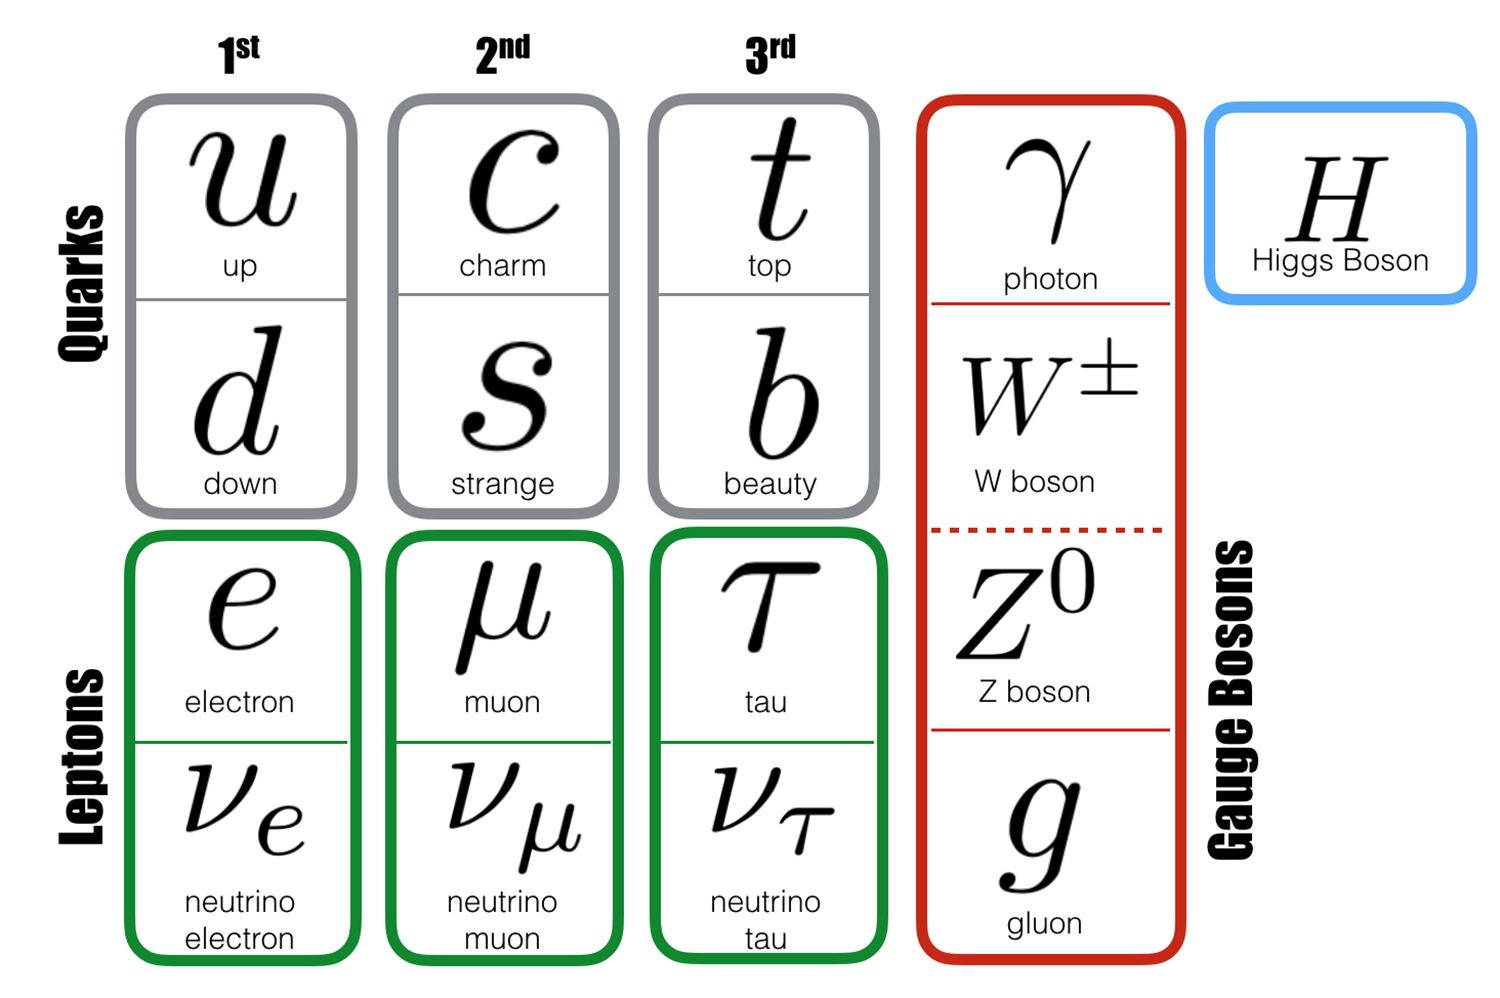
\includegraphics[width=\linewidth]{figs/SM.png}
  \caption{Summary of elementary SM particles. The first three columns give
           the three generations of matter particles. Image taken
           from the Physics Institute at University of
           Zurich~\cite{zurich_SM}.}
  \label{fig:SM}
\end{figure}

Figure~\ref{fig:SM} gives a schematic overview of the SM.
In the first three columns are all the known matter particles.
Matter particles can be divided into\index{quark} {\it quarks}
and\index{lepton} {\it leptons}. Quarks make up so-called {\it hadrons},
the most familiar of which to you would be protons and neutrons; for
example a proton is made of two up quarks and a down quark. Quarks can feel the
strong force, the EM force, the weak force, and the Higgs. 
Leptons differ from quarks in that they do not feel the strong force; moreover
we do not believe the neutrinos feel\footnote{Nevertheless, they appear to be
massive. How neutrinos acquire their masses is an area of active research in
particle physics.} the Higgs. The electron is the lepton most
familiar to you. Quarks and leptons can be divided into three\index{generation}
{\it generations}, which are indicated at the top of each column.
Masses distinguish\footnote{The later generations are heavier than the earlier
generations. This is not true for neutrinos, whose mass ordering has yet to be
determined.} the various generations; for instance the top quark is
heavier than the charm, which is heavier than the up, even though they all have
electric charge $+2/3$.

The fourth column we find the gauge bosons, which\index{mediate} 
{\it mediate} the fundamental forces, i.e. we believe that particles feel forces
by exchanging gauge bosons. For example, the photon mediates the EM interaction.
When two electrons repel from each other, from the modern perspective of
particle physics, this occurs because they are exchanging photons.
As discussed in \secref{sec:groupsMatter}, gauge bosons are a physical
manifestation of underlying symmetries. The photon and $W$ and $Z$ bosons
are manifestations of a combined $\SU(2)\times\U(1)$ symmetry. Meanwhile the
gluon is a manifestation of an $\SU(3)$ gauge symmetry.

Sometimes it is useful to focus on only part of the SM. In the case of lattice
calculations, one reason to do this is that the more particles you add to a
simulation, the more expensive it becomes. The strong force is also special
because it has a well-defined {\it continuum limit}, which we will discuss in
\chref{ch:LFT}. For these reasons, lattice simulations focus on systems with
only quarks and gluons. This is the realm of QCD, and lattice simulations of QCD
are usually called lattice QCD (LQCD). 

\subsection{Fields}\label{sec:fields}

As already mentioned in \secref{sec:SR}, a field is some math object defined on
all space and time, and I gave the simple example of temperature as a scalar
field. From the perspective of modern physics, all particles are understood as
manifestations of underlying fields. Hence there is a photon field, and electron
field, and so on. Fields whose manifestations are quarks and leptons are called
{\it matter fields}\index{field!matter}. Similarly, fields whose manifestations
are gauge bosons are {\it gauge fields}\index{field!gauge}.

\begin{figure}
  \centering
  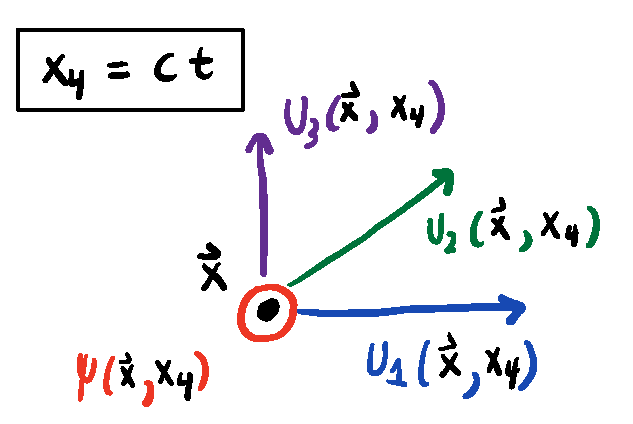
\includegraphics[width=0.6\linewidth]{figs/fields.pdf}
  \caption{A schematic drawing of some fields associated with a space-time point
           $\fvec{x}=(\vec{x},x_4)$. In this theory there is a matter field
           $\psi(\fvec{x})$ and a gauge field $U_\mu(\fvec{x})$ with four
           components labeled by $\mu$, $1\leq\mu\leq4$.
           We can only show three spatial components (directions) of the gauge field 
           $U_1(\fvec{x})$, $U_2(\fvec{x})$, and $U_3(\fvec{x})$.}
  \label{fig:fields}
\end{figure}

Fields play an extremely important role in the formalism of the SM, which is
usually called {\it quantum field theory} QFT. Introducing matter fields with a
particular mathematical structure allows them to be compatible with special
relativity; in fact the whole QFT formalism was born out of an attempt to make
quantum mechanics compatible with special relativity. They also are important in
another way: they proffer an explanation why particles are exactly identical.
Indeed the fact that all photons are indistinguishable, all electrons are
indistinguishable, and so on, is a conclusion one reaches when learning
statistical physics.
Matter fields are introduced as a math object called a {\it spinor}, which can
be expressed as a complex vector. Gauge fields, meanwhile, can be expressed as
matrices ``that point in a direction", i.e. in a 4-$d$ space-time, there are
four gauge fields associated to each space-time point. A schematic
representation of this is given in \figref{fig:fields}.

Let us gain a bit more geometric intuition for these gauge matrices. We will
start with the gauge group $\U(1)$ and work our way up in complexity.
Recall from \secref{sec:groupsMatter} that $\U(1)$ could be identified with the
set of rotations of a circle. Hence, for a theory that has an underlying gauge
group $\U(1)$, you can imagine at each point in space and time something
like \figref{fig:fields}, where each colored arrow could be any point on a
circle\footnote{The arrows in the figure are just supposed to emphasize that
there are four matrices per space-time point, one associated with each direction
$x$, $y$, $z$, and $t$. In the case of $\U(1)$, you can at least schematically
think of each gauge matrix as a circle attached to each arrow. Generically
speaking, varying the gauge field is equivalent to spinning all the circles
attached to all the arrows of every space-time point.}.

The next-most interesting gauge group is $\SU(2)$. It can be represented as
\begin{equation}
\SU(2)=\left\{
\left(\begin{array}{cc}
          a+ib   & -c+id  \\
          c+id   &  a-ib  \\
            \end{array}\right)\suchthat a,b,c,d\in\R \right\}.
\end{equation} 
One property of $\SU(N)$ matrices, $N\in\N$, is that they have determinant 1.
This leads to the constraint
\begin{equation}
a^2+b^2+c^2+d^2=1,
\end{equation}
which is the equation for the unit hypersphere in four dimensions, often 
denoted\footnote{In general, $S^m$ is the unit hypersphere in $m+1$ dimensions.}
$S^3$. We can therefore think of $\SU(2)$ elements as points on $S^3$.

The group that is actually relevant for strong interactions is $\SU(3)$. Because
of the above two situations, I always sort of figured that $\SU(3)$ could be
thought of as a point on $S^8$. Unfortunately this is not the case. Still,
$\SU(3)$ elements are characterized completely by eight angles, in such a way
that you can sort of imagine it as two hyperspherical surfaces $S^5$ and $S^3$
somehow\footnote{I guess the correct statement is something like ``$\SU(3)$
is the total space of an $S^3$ fibration over $S^5$." I don't really know what
that means, hence the entangled hyperspheres metaphor. I guess if you eventually
choose to take differential geometry, you will learn.} entangled with each other.


%The theoretical framework underlying the SM is an example of a Quantum
%Field Theory (QFT). QFTs are consistent with both quantum mechanics and
%relativity. Lattice gauge theories are a kind of QFT; therefore it is
%important for the reader to know a little bit about them. There are a lot
%of different resources one can use to learn about QFT; for example when I was a
%grad student I used Peskin and Schroeder~\cite{peskin_introduction_1995}
%and Srednicki~\cite{srednicki_quantum_2007}.
%Nowadays there are also some very high quality lectures on YouTube,
%for instance a series by Tong~\cite{tongQFT}, which I found had some other nice
%introductory remarks.
%A timeline of particle discoveries can be found in
%Ref.~\cite{wiki_particle_discoveries}. Another detailed historical overview
%of the SM is given in Chapter 1 of Ref.~\cite{griffiths_introduction_2007}.

\section{Further reading}

At some point in your career, you should learn each of these subjects in some
careful detail. Here I collect some resources that I found helpful when I was an
undergraduate. 
\begin{itemize}
  \item Electrodynamics: For this subject, the standard favorite is
Griffiths's {\it Introduction to electrodynamics}~\cite{Griffiths:1492149}.
You will see that Griffiths makes a lot of nice physics books at the
undergraduate level.
  \item Special and general relativity:
A good starting point is Moore's {\it Six Ideas that Shaped Physics: Unit
R}~\cite{moore2002six}. A nice next step would be {\it Relativity, Gravitation,
and Cosmology: A Basic Introduction} by Cheng~\cite{alma997111578601771}.
  \item Quantum mechanics:
Most classes use Griffiths's {\it Introduction of Quantum
Mechanics}~\cite{griffiths_introduction_2005}. This is a nice book, and I especially enjoy
its discussion at the end of Bell's inequality\footnote{Which you may want to
read at some point, seeing as the 2022 Nobel prize in physics was the
experimental verification of this.}. Still my favorite is Shankar's
{\it Principles of Quantum Mechanics}~\cite{Shankar:102017}, which contains an
extremely helpful mathematical introduction.
  \item Thermodynamics:
Shroeder's {\it An Introduction to Thermal
Physics}~\cite{schroeder2021introduction} is the only book at the undergraduate
level I have tried.
  \item Particle physics:
{\it Introduction to Elementary Particles} by
Griffiths~\cite{griffiths_introduction_2007} explains some of the basic ideas of
modern particle physics and has a nice history in the beginning. Thomson's
{\it Modern Particle Physics}~\cite{thomson_modern_2013} is certainly accessible to an advanced
undergraduate and more up-to-date, including for instance an elementary
explanation of the Higgs mechanism.
\end{itemize}

\section*{Exercises}

For Exercises (1-5), write a Python function that:
\begin{enumerate}
    \item converts between [mi] and [m];
    \item converts between [s], [min], [h], and [y];
    \item converts between [lb] and [kg], assuming you’re close to the earth’s surface;
    \item given an object with some mass and height above the earth’s surface, can 
          calculate how much gravitational potential energy in [J] the object has; and
    \item converts between [m] and [ly].
    \item A tank weighs about 140,000 [lbs]. Use your program from problem (4) 
          to calculate how much gravitational potential energy in [J] the tank has when 
          it’s 1 [mi] off the ground.
    \item Assuming an apple has a mass of 100 [g], calculate its rest mass energy.
    \item Suppose you could magically convert 100\% of an apple’s rest mass into energy, 
          and then use that energy to lift a tank off the ground. How far off the 
          ground could you lift it?
    \item Write a python script that converts between [MeV] and [fm$^{-1}$].
          Also write a script that converts between [fm] and [MeV$^{-1}$].
    \item Working in the natural unit system, express the units of power, pressure,
          and momentum as a power of [MeV]. Repeat for [fm].
    \item What is your height in [MeV$^{-1}$]?
    \item Use \equatref{eq:massp} to determine the proton mass in [kg].
    \item Show that \equatref{eq:Tsun} is correct.
\end{enumerate}

\bibliographystyle{unsrtnat}
\bibliography{bibliography}
